
%%% Local Variables:
%%% mode: latex
%%% TeX-master: t
%%% End:

\chapter{宏观模型更新}

\section{宏观模型研究内容}
宏观交通模型是一体化交通模型的基础,模型范围为深圳全市域,模拟城市
交通系统中主要交通方式的运行情况,具体包括私人交通系统中的小汽车、出租
车和货车系统,以及公交系统中的常规公交和轨道系统,并且预留有轨电车、
BRT 等系统。宏观交通模型基于“四阶段”理论,标定了城市社会经济和土地
利用-交通运行的交通需求模型,进行现状交通需求的模拟和未来交通需求的预测。

宏观交通模型主要作为第一层次的交通研究辅助工具,建模估算整个深圳市
交通运输需求,为土地开发利用和综合交通运输体系政策和规划提供评价。主要
功能是预测交通走廊和主要道路的交通量、预测主要公共交通设施流量、测试交
通政策效果。同时宏观交通模型也为第二层次或第三层次的交通研究提供基础模
型,这两个层次的模型可在此基础上针对研究问题进行进一步的编辑,输入更多
的信息,从而满足这两个层次研究的需求。

\subsection{模型范围}
模型范围为全深圳市域。全市交通小区共 1137 个,其中普通小区 1071 个,
火车站、机场、港口、口岸、国省道、规划城际轨道出入口等特殊交通小区 66个。全市模型交通小区范围如
图\ref{fig:模型交通小区示意图}所示。

\begin{figure}[ht]
  \centering
  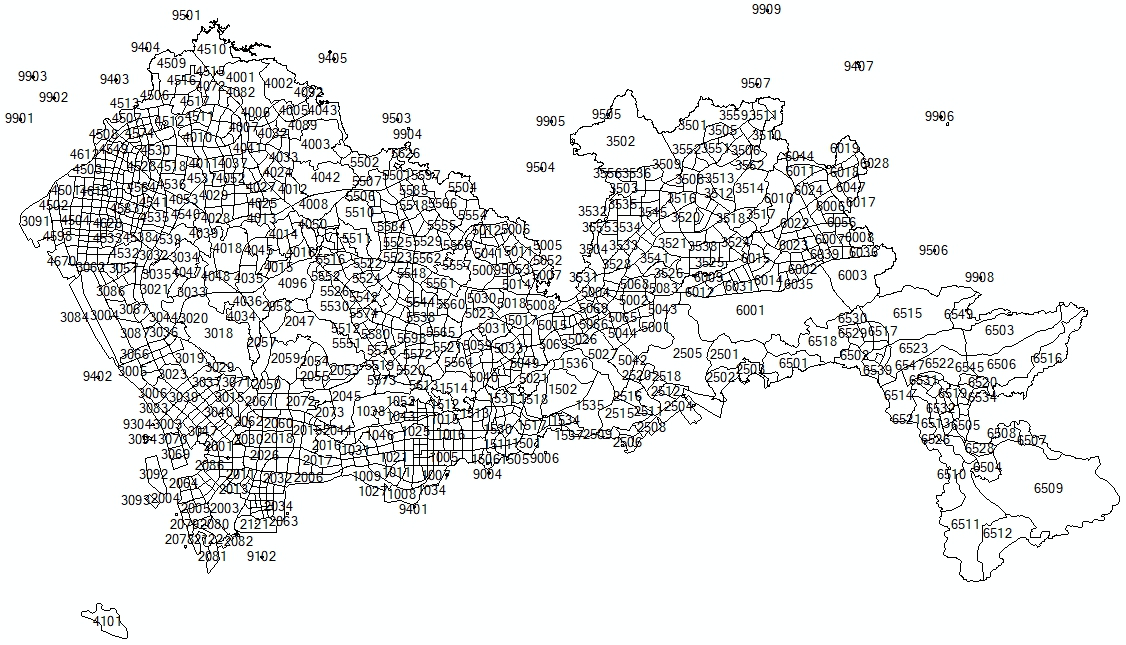
\includegraphics[width=0.9\textwidth]{chp04_模型交通小区示意图.jpg}
  \caption{模型交通小区示意图\label{fig:模型交通小区示意图} }
\end{figure}

\subsection{模型内容}
宏观模型包括基年模型、现状模型和规划模型三种类型的模型。每种模型的
数据基础、建模方法和功能不尽相同。

\smalltitle{基年模型}
基年模型是宏观模型体系中的基础模型。基年模型的功能是通过一系列数学
模型,建立地区社会经济数据和土地利用数据与地区交通运行情况的运算关系,
并且假定这一关系在短时间内相对稳定,因此根据此运算关系可以推算目前交通
运行情况和预测未来交通运行情况。

基年模型以交通规划“四阶段法”为基础,包括需求预测模型、货运模型及
特殊吸引点等子模型。建模过程首先对每个子模型进行评估,通过分析居民出行
特征以及其他交通出行相关数据构建每个子模型输入量与输出量的数据关系。在
运行模型其他部分之前,要根据基准年数据对每个子模型进行校核。

由于宏观模型的基础调查数据为居民出行调查数据,因此基年模型基于
2010 年深圳市居民出行大调查数据,基准年为 2010 年。更新周期取决于核心的
数据来源居民出行调查的开展周期,约为 5 年。 2016 年 11 月 15 日至 2017 年 1
月 15 日,深圳市开展了第六次全市范围内的大规模居民出行调查,本次模型更新在此新数据基础上
开展了部分模块的参数校核及更新工作。

\smalltitle{现状模型}
现状模型是模拟当年通道交通需求及道路运行情况的模型。其主要应用于近
期市域层面较大项目的方案测试与评价。

为了更好的模拟每一年的交通运行情况,现状模型基于基年模型的框架和参
数,在此基础上输入现状土地利用、交通网络数据,形成现状模型,并根据当年
的道路交通流量检测值、公共交通刷卡数据等, 需求模型得到的 OD 矩阵进行检
验与调整。现状模型反应当年交通运行状况,每年更新一次。

\smalltitle{规划模型}
规划模型是预测规划年的综合交通需求结构和主通道交通需求及道路运行
情况的模型。应用于市域战略性规划、用地结构与空间布局规划、较大交通基础
设施的布局规划。

规划模型遵循基年模型建立的运算关系,输入规划年的社会经济和土地利用
数据,从而预测未来特征年交通系统需求结构和整体交通运行情况。按照目前深
圳市城市土地利用规划的阶段,规划年模型分为 2020 年, 2030 年, 2040 年。规
划模型的核心输入量为土地利用数据、规划年综合交通网络和基年模型建立的运
算关系。一般根据土地利用数据及综合交通规网络(主要是轨道网络)的更新周
期而更新。

\section{宏观模型架构及更新方法}
\subsection{宏观模型架构}
模型整体架构采用四阶段交通模型,框架图如图\ref{fig:chp04_宏观交通模型框架图}所示。

\begin{figure}[ht]
  \centering
  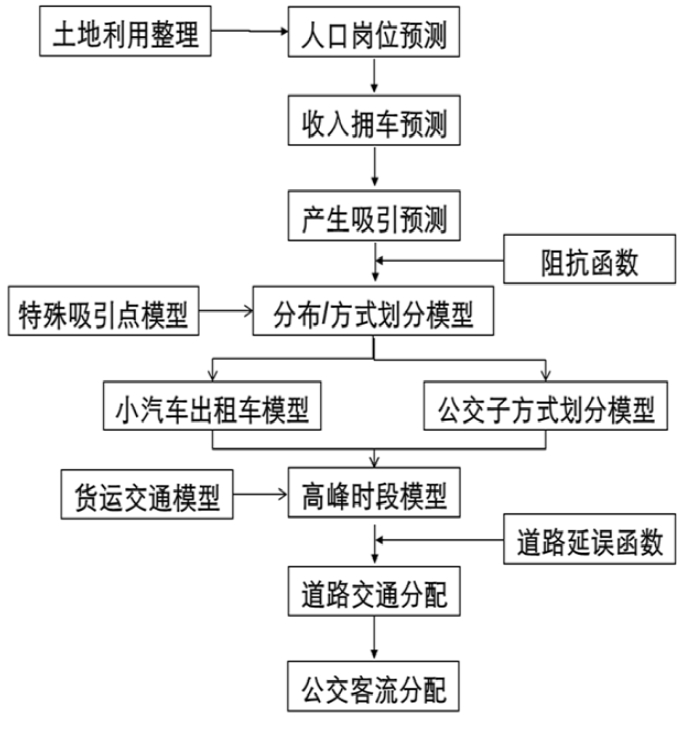
\includegraphics[width=0.5\textwidth]{chp04_宏观交通模型框架图.jpg}
  \caption{宏观交通模型框架图\label{fig:chp04_宏观交通模型框架图} }
\end{figure}

宏观交通模型模块主要包括:
\begin{para}
\item[收入模型] 通过社会经济总体预测数据和小区用地类型,计算小区平均收入
\item[拥车模型] 以小区平均收入为核心变量,计算小区拥车情况分布
\item[出行生成] 通过分目的生成模型和分目的吸引模型,计算得到分目的的
交通产生量和吸引量
\item[出行分布] 对于不同目的的机动化出行产生吸引量,分别通过双约束重力模型,
计算得到不同目的的机动化出行 OD
\item[方式预划分] 对于不同目的的交通产生吸引量,分别通过转移曲线模型,
将出行划分为慢行出行和机动化出行
\item[方式划分] 对于不同目的的机动化出行 OD,分别通过 Logit 模型计算得
到不同出行目的的公交 OD、客车 OD 和出租车 OD
\item[公交子方式划分] 对于不同目的公交 OD 进一步分为常规公交 OD 和轨
道交通 OD,使用 Logti 模型来计算
\item[外部及特殊吸引点模型] 对于主要对外通道和枢纽中的跨市域出行和旅
客出行仿真
\item[出租车模型] 调整出租车空载和调查产生的出租车矩阵误差
\item[货车模型] 根据工业和仓储用地分布,计算货车出行
\item[交通分配] 对于客流 OD 通过客流分配模型,进行交通分配;对于车流
OD 通过均衡模型,进行交通分配 
\end{para}

\subsection{宏观模型特点}
\smalltitle{精细化建模方法}
精细化人群分类:根据深圳市人口特点,首先将人口划分为家庭户和集体户
人口。建立收入模型和拥车模型,根据收入和拥车再次细分人群,精细化模拟不
同人群的出行特征。

精细化细化网络:模型包括 85478 个路段, 869 条常规公交线路, 10016 个
公交站点。并对立交、主辅道等复杂拓扑关系进行了模拟。

精细化费用模型:根据深圳市公共交通票价体系,建立了一套公共交通票价
体系,真实模拟票价,从而提高了模型精度,且支持各种票价敏感性测试。

精细化成果输出:轨道客流预测结果可以获得从网络、线路到站点不同层面
的数据,支持轨道网络规划、轨道交通建设规划、轨道线路交通详细规划、轨道
线路工可研究、轨道线路初步设计研究等不同深度的轨道相关规划。

\smalltitle{动态大数据校核模型}
采用刷卡数据、公交 GPS 数据、出租车 FCD 数据、车牌识别数据等动态大
数据标定和校核模型。克服了以往仅采用居民出行调查数据标定参数的诸多局限
性。采用 FCD 数据建立了出租车空驶模型,提高了模型精度。

\smalltitle{良好的人机交互模式}
模型设置了易读的运行界面,操作方便。模型主要参数及数据存储在 Excel
中,克服了传统模型的“黑匣子”。设置常用图表模板。针对规划应用,设计了
几十种常用图表模板,可以快捷方便的生成图表,并保证了图表的标准化格式。

\subsection{模型应用流程}
宏观模型模型应用的流程为:
\begin{nbeae}
\item 在 PTV 软件中编辑更新道路网、轨道网络等综合交通网络;
\item 在 Excel 文件“ Parameters”中更新人口、土地利用、对外客运量等数据
\item 在 PTV 模型中运行已设置好的 Procedure,如图\ref{fig:chp04_PTV设置的procedure.jpg}所示:
\end{nbeae}

\begin{figure}[ht]
  \centering
  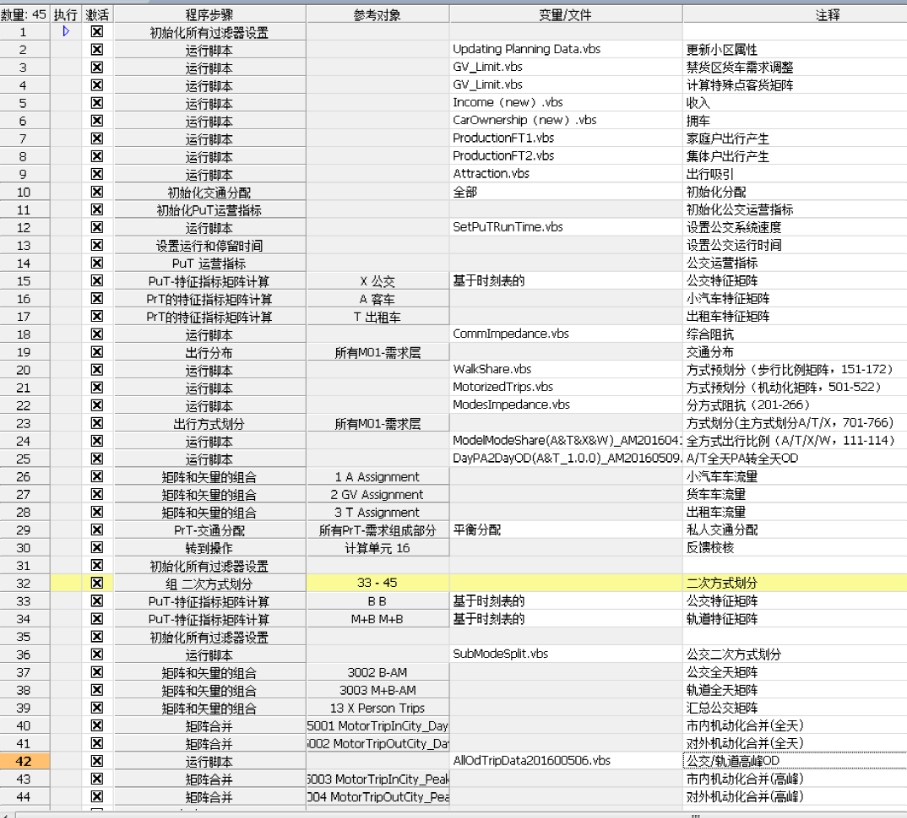
\includegraphics[width=0.8\textwidth]{chp04_PTV设置的procedure.jpg}
  \caption{PTV设置的 procedure\label{fig:chp04_PTV设置的procedure.jpg} }
\end{figure}

\begin{cit}
\item \qd{第1部分}:编号 2,更新小区人口和土地利用数据,如果小区数据没有
更新则不需要运行;
\item \qd{第2部分}:编号 3-4,货车和外部矩阵计算;
\item \qd{第3部分}:编号 5-9,出行生成模型计算;
\item \qd{第4部分}:编号 10-18, 综合阻抗计算;
\item \qd{第5部分}:编号 19,出行分布模型计算;
\item \qd{第6部分}:编号 20-24,方式划分模型计算;
\item \qd{第7部分}:编号 25,出行时辰模型计算;
\item \qd{第8部分}:编号 26-29,矩阵计算和私人交通分配;
\item \qd{第9部分}:编号 30,循环条件设置,不满足条件则至计算综合阻抗开
始循环;
\item \qd{第10部分}:编号 32-36, 公交二次方式划分。
\item \qd{第11部分}:编号 37-42, 公交及轨道全天 OD、高峰 OD 计算。
\item 设置完成后,选择需要计算的步骤,将执行开始箭头移到第一步需要运
算的步骤;
\item 点击运行按钮,运算整个计算程序。
\end{cit}

\subsection{模型矩阵说明}
深圳需求模型计算过程中,需要 242 个矩阵参与计算,矩阵的位置和功能固
定,在计算过程中根据编号读取和填写数值。

\smalltitle{需求矩阵说明}
需求模型参与计算的矩阵中包括 130 个需求矩阵,作为模型计算结果存储,
以及最后分配的输入量,说明如下:

\renewcommand{\arraystretch}{0.8}
\begin{longtable}[c] {|C{0.1\textwidth}|>{\baselineskip=14pt}m{0.67\textwidth}|C{0.12\textwidth}|} 
  \caption{需求矩阵说明\label{tbl:需求矩阵说明}}
  \hline
  \multicolumn{1}{|c|}{\bfseries 矩阵编号} & \multicolumn{1}{c|}{\bfseries 说明} & 
  \multicolumn{1}{c|}{\bfseries 备注} \\\hline
1 & 分配小汽车矩阵 & 单位:车 \\\hline
2 & 分配货车矩阵 & 单位:车 \\\hline
3 & 分配出租车矩阵 & 单位:车 \\\hline
4 & 分配公交矩阵 & 单位:人 \\\hline
11 & 需求模型预测市内家庭户集体户小汽车出行矩阵 & 单位:人 \\\hline
12 & 需求模型预测市内家庭户集体户出租车出行矩阵 & 单位:人 \\\hline
13 & 需求模型预测市内家庭户集体户公交出行矩阵 & 单位:人 \\\hline 
14 & 需求模型预测市内家庭户集体户步行出行矩阵 & 单位:人 \\\hline
15 & 市内货车矩阵 & 单位:车 \\\hline
16 & 对外通道进出深圳货车矩阵 & 单位:车 \\\hline
17 & 特殊吸引点进出深圳货车矩阵 & 单位:车 \\\hline
31 & 对外通道进出深圳小汽车矩阵 & 单位:车 \\\hline
32 & 特殊吸引点进出深圳小汽车矩阵 & 单位:车 \\\hline
33 & 特殊吸引点进出深圳公交矩阵 & 单位:人 \\\hline
51 & 全方式市内家庭户集体户出行矩阵 & 单位:人 \\\hline
52 & 全方式市内家庭户出行矩阵 & 单位:人 \\\hline
53 & 全方式市内集体户出行矩阵 & 单位:人 \\\hline
54 & 机动化市内家庭户集体户出行矩阵 & 单位:人 \\\hline
55 & 机动化市内家庭户出行矩阵 & 单位:人 \\\hline
56 & 机动化市内集体户出行矩阵 & 单位:人 \\\hline
501-522 & 方式预划分模型计算结果,22 类模型机动化矩阵 & 单位:人 \\\hline
601-622 & 出行分布模型计算结果,22 类模型的全方式矩阵 & 单位:人 \\\hline
701-766 & 方式划分计算结果,22 类模型小汽车、出租车和公交矩阵 & 单位:人 \\\hline
\end{longtable}

\smalltitle{阻抗矩阵说明}
需求模型参与计算的矩阵中包括 112 个阻抗矩阵,作为模型的输入量,说明如下:

\renewcommand{\arraystretch}{0.8}
\begin{longtable}[c] {|C{0.1\textwidth}|>{\baselineskip=14pt}m{0.65\textwidth}|C{0.15\textwidth}|} 
  \caption{阻抗矩阵说明\label{tbl:阻抗矩阵说明}}
  \hline
  \multicolumn{1}{|c|}{\bfseries 矩阵编号} & \multicolumn{1}{c|}{\bfseries 说明} & 
  \multicolumn{1}{c|}{\bfseries 备注} \\\hline
101 & 综合阻抗矩阵 & 单位:分钟 \\\hline
102 & 小汽车综合阻抗矩阵 & 单位:分钟 \\\hline
103 & 出租车综合阻抗矩阵 & 单位:分钟 \\\hline
104 & 公交综合阻抗矩阵 & 单位:分钟 \\\hline
105 & 步行综合阻抗矩阵 & 单位:分钟 \\\hline
111 & 小汽车依据出行产生小区的分担率矩阵 &  \\\hline
112 & 出租车依据出行产生小区的分担率矩阵 & \\\hline
113 & 公交依据出行产生小区的分担率矩阵 & \\\hline
114 & 步行依据出行产生小区的分担率矩阵 & \\\hline
121 & 小汽车行程时间矩阵 & 单位:分钟  \\\hline
122 & 小汽车出行距离矩阵 & 单位:公里 \\\hline
123 & 出租车行程时间矩阵 & 单位:分钟 \\\hline
124 & 出租车出行距离矩阵 & 单位:公里 \\\hline
125 & 公交在车时间矩阵 & 单位:分钟 \\\hline
126 & 公交换乘等待时间矩阵 & 单位:分钟 \\\hline
127 & 公交步行时间矩阵 & 单位:分钟 \\\hline
128 & 公交起点小区至起点站点 connectors 步行时间矩阵 & 单位:分钟 \\\hline
129 & 公交终点小区至终点站点 connectors 步行时间矩阵 & 单位:分钟 \\\hline
130 & 公交平均换乘次数的矩阵 & 单位:次 \\\hline
131 & 公交费用矩阵 & 单位:元 \\\hline
149 & 小区内出行距离 & 单位:公里 \\\hline
150 & 包括小区内出行距离的出行距离矩阵 & 单位:公里 \\\hline
151-172 & 方式预划分模型计算结果, 22 类模型步行比例矩阵 & \\\hline
201-266 & 方式划分模型计算输入矩阵, 22 类模型方式划分小汽车、出
租车和公交的阻抗矩阵 & 单位:分钟 \\\hline
301 & 货车外部小区权重矩阵 & \\\hline
302 & 客车外部小区权重矩阵 & \\\hline
\end{longtable}

\subsection{宏观模型更新流程}
宏观模型更新包括现状年模型更新及规划年模型更新。宏观模型更新的主要
内容包括输入条件更新、大数据更新矩阵。输入条件更新包括人口及土地利用数
据更新、道路网络更新、公交及轨道网络更新、小汽车保有量、对外客货运总量
等数据更新。 矩阵更新主要指根据 GPS 数据、轨道刷卡数据分析得到的出租车
矩阵及轨道进出站 OD 矩阵。 鉴于本次更新之前,开展了《 2017 年深港莞惠跨
界交通调查》项目,获得了口岸、机场等枢纽分时段 OD,并根据手机信令数据、
境界线调查数据获得分时段分方式 OD,因此主要更新了对外交通模型。图\ref{fig:chp04_现状模型更新流程}
是现状模型更新的流程。

\begin{figure}[ht]
  \centering
  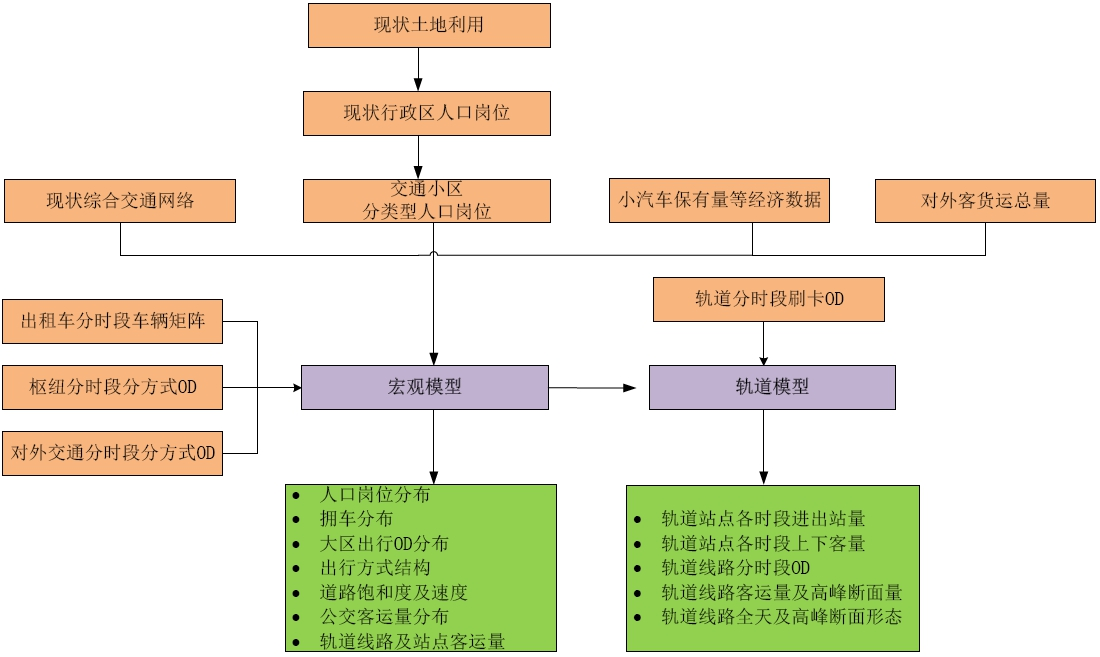
\includegraphics[width=0.9\textwidth]{chp04_现状模型更新流程.jpg}
  \caption{现状模型更新流程\label{fig:chp04_现状模型更新流程} }
\end{figure}

规划年模型更新主要为输入条件更新,即规划年人口、岗位、土地利用、综
合交通网络、小汽车保有量等社会经济数据、收费等政策量化值。 输入数据更新
后,运行交通模型,更新相关输出图表,详见图\ref{fig:chp04_规划年模型更新流程}所示。

\begin{figure}[ht]
  \centering
  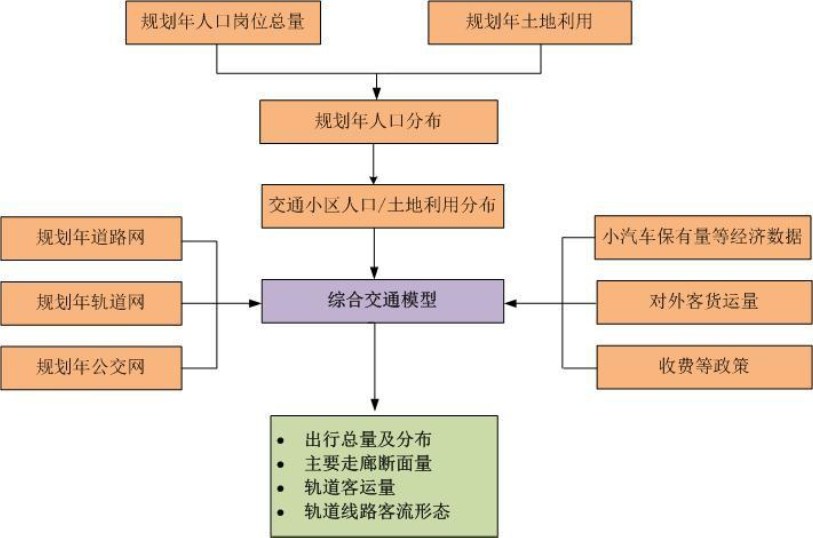
\includegraphics[width=0.7\textwidth]{chp04_规划年模型更新流程.jpg}
  \caption{规划年模型更新流程\label{fig:chp04_规划年模型更新流程} }
\end{figure}

\section{模型输入条件更新}
\subsection{综合网络更新}
交通模型综合交通网络包括道路网络、常规公交网络、轨道交通网络、长途
大巴网络。图\ref{fig:chp04_模型综合网络}是综合交通网络的详细结构。

\begin{figure}[ht]
  \centering
  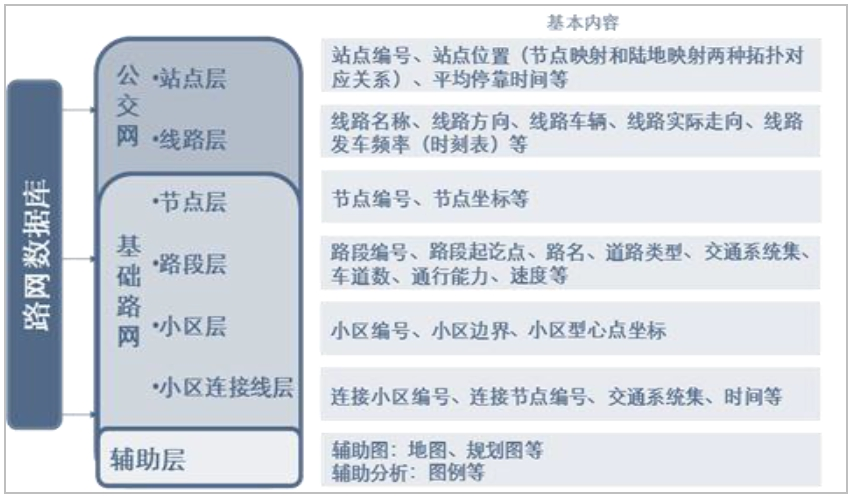
\includegraphics[width=0.7\textwidth]{chp04_模型综合网络.jpg}
  \caption{模型综合网络\label{fig:chp04_模型综合网络} }
\end{figure}

道路数据更新的技术方法是:以数据及查询系统更新的路网及更新标志为基
础,在 PTV 软件中手动更新。更新的流程包括更新道路形状、更新道路节点、
更新道路属性、调整公交线路(部分道路有公交线路经过)和质量检查五个环节。
PTV 软件中自带程序可以检查是否有独立点、断头路等网络拓扑错误。

常规公交与轨道网络采用批量导入 GIS 文件的方式更新。 截止 2017 年底常
规公交运营线路 1110 条,站点总数 12755 个。 现状运营轨道网络与上一年度无
变化。 规划年轨道网络根据《深圳市轨道网络规划( 2016-2035)》进行了更新。
规划远景全市城市轨道共 33 条线路,总长约 1335 公里(含弹性发展线路 112 公
里),其中市域快线 9 条,总长 494.5 公里,普速线路 24 条,总长 840.5 公里,
形成了城际铁路、市域快线、普速线路三层次的轨道线网体系。

\begin{figure}[!htpb]
  \centering
  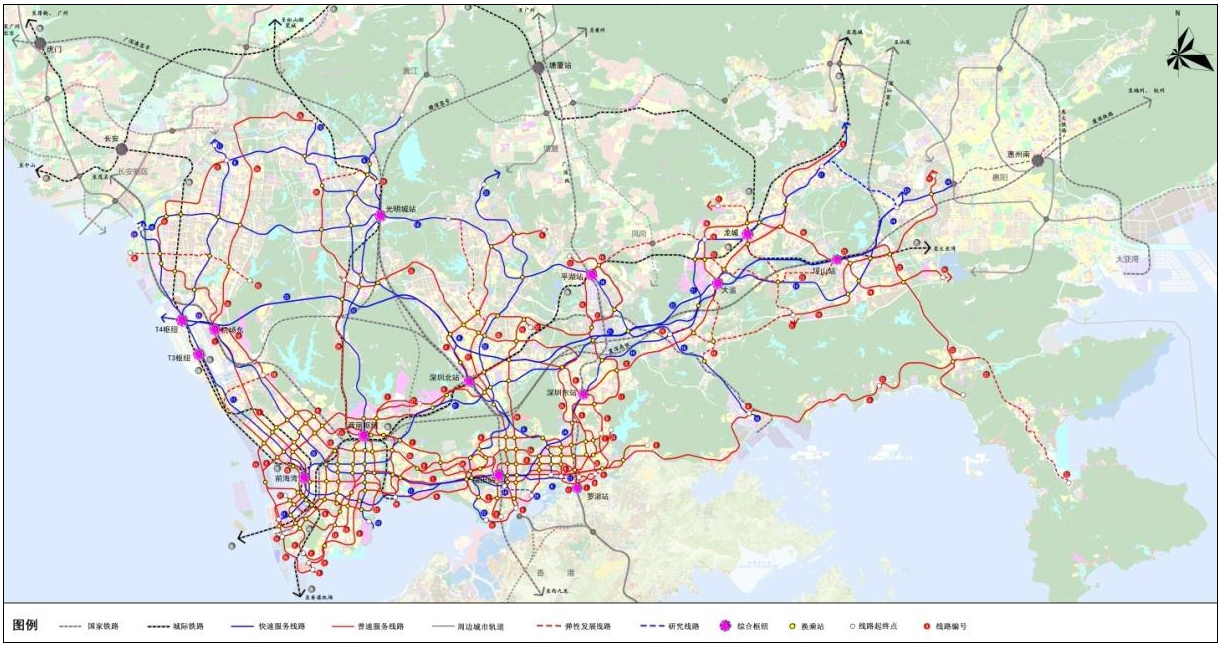
\includegraphics[width=\textwidth]{chp04_深圳市轨道线网总体布局规划图.jpg}
  \caption{深圳市轨道线网总体布局规划图\label{fig:chp04_深圳市轨道线网总体布局规划图} }
\end{figure}

\subsection{人口及土地利用数据更新}
\subsubsection{根据 2016 年建筑物普查更新现状年土地利用}
根据 2016 年现状建筑物普查更新现状年土地利用。全市现状建筑量约 10.8
亿平米,比 2014 年增加 3190 万平米。表\ref{tbl:现状各区建筑开发量}是分行政区的现状建筑开发量。

\renewcommand{\arraystretch}{0.8}
\begin{longtable}[c] {|C{0.08\textwidth}|C{0.1\textwidth}|C{0.1\textwidth}|C{0.1\textwidth}|
C{0.1\textwidth}|C{0.1\textwidth}|C{0.1\textwidth}|C{0.1\textwidth}|} 
  \caption[现状各区建筑开发量]{现状各区建筑开发量(万平米)\label{tbl:现状各区建筑开发量}}
  \hline
  \multicolumn{1}{|c|}{\bfseries 行政区} & \multicolumn{1}{c|}{\bfseries 居住} & 
  \multicolumn{1}{c|}{\bfseries 私宅} & \multicolumn{1}{c|}{\bfseries 商业} & 
  \multicolumn{1}{c|}{\bfseries 办公} & \multicolumn{1}{c|}{\bfseries 工业} &
  \multicolumn{1}{c|}{\bfseries 其他} & \multicolumn{1}{c|}{\bfseries 合计} \\\hline

罗湖 & 3777.7 & 666.4   & 719.6  & 713.0  & 351.6   & 337.2  & 6565.5  \\\hline
福田 & 5304.2 & 747.4   & 2618.4 & 69.5   & 365.0   & 899.6  & 10004.1 \\\hline
南山 & 6263.1 & 844.1   & 889.5  & 1992.1 & 1517.7  & 854.0  & 12360.5 \\\hline
盐田 & 846.9  & 105.3   & 172.6  & 195.8  & 320.6   & 158.7  & 1799.7  \\\hline
宝安 & 9052.2 & 5736.6  & 1442.7 & 548.8  & 8281.3  & 732.7  & 25794.4 \\\hline 
光明 & 1626.4 & 1915.7  & 242.6  & 105.0  & 2934.5  & 165.4  & 6989.7  \\\hline
龙华 & 4842.4 & 3697.2  & 669.7  & 233.3  & 3736.9  & 287.7  & 13467.2 \\\hline
龙岗 & 9229.0 & 5670.1  & 1444.5 & 461.5  & 6581.9  & 682.2  & 24069.2 \\\hline
坪山 & 1461.2 & 1293.6  & 136.1  & 90.1   & 2026.8  & 166.6  & 5174.3  \\\hline
大鹏 & 615.6  & 510.1   & 79.8   & 22.6   & 389.6   & 91.0   & 1708.8  \\\hline
合计 & 43018.7& 21186.6 & 8415.4 & 4431.5 & 26505.8 & 4375.1 & 107933.1\\\hline 
\end{longtable}

\renewcommand{\arraystretch}{0.8}
\begin{longtable}[c] {|C{0.08\textwidth}|C{0.1\textwidth}|C{0.1\textwidth}|C{0.1\textwidth}|
C{0.1\textwidth}|C{0.1\textwidth}|C{0.1\textwidth}|C{0.1\textwidth}|} 
  \caption[2015 年建筑开发增量]{2015年建筑开发增量( 万平米)\label{tbl:2015 年建筑开发增量}}
  \hline
  \multicolumn{1}{|c|}{\bfseries 行政区} & \multicolumn{1}{c|}{\bfseries 居住} & 
  \multicolumn{1}{c|}{\bfseries 私宅} & \multicolumn{1}{c|}{\bfseries 商业} & 
  \multicolumn{1}{c|}{\bfseries 办公} & \multicolumn{1}{c|}{\bfseries 工业} &
  \multicolumn{1}{c|}{\bfseries 其他} & \multicolumn{1}{c|}{\bfseries 合计} \\\hline

罗湖 & 33.1  & 40.6  & 100.5  & 47.5   & 3.4  & 50.0  & 275.0 \\\hline
福田 & 166.9 & -23.9 & 1808.3 & -1769.8& 18.7 & 145.5 & 345.8 \\\hline
南山 & 102.2 & -4.7  & 176.8  & 366.2  & -37.8& 0.0   & 602.6 \\\hline
盐田 & -24.2 & 0.0   & 62.3   & 10.3   & 18.5 & 10.4  & 77.2  \\\hline
宝安 & 477.2 & 34.7  & 107.3  & 33.1   & -42.2& 77.4  & 687.5 \\\hline
光明 & 104.8 & -11.8 & 37.0   & 25.3   & -4.5 & 31.2  & 182.2 \\\hline
龙华 & 233.8 & -24.1 & 5.8    & 56.0   & -28.6& 21.1  & 264.0 \\\hline
龙岗 & 295.9 & -66.5 & 41.4   & 120.0  & -35.2& 70.4  & 426.1 \\\hline
坪山 & 141.9 & -10.9 & -0.5   & 49.2   & 64.0 & 38.9  & 282.5 \\\hline
大鹏 & 47.2  & -2.9  & -0.1   & 0.0    & -0.9 & 4.2   & 47.6  \\\hline
合计 & 1578.7& -69.6 & 2338.8 & -1062.5& -44.6& 449.3 &3190.2 \\\hline
\end{longtable}

\subsubsection{更新规划年土地利用}
现状建筑物普查数据,结合土地利用规划(新区规划、法定图则、发展单元、
城市更新、详细蓝图、个案调整等法定规划,更新到 2015 年 12 月),整合得到
远期的规划一张图。依据整合的远期土地利用规划一张图,规划年土地利用包括
40701 个地块(不含非建设用地),各地块按 GIS 格式进行信息处理,含用地功
能、容积率、开发时序( 2020 年, 2030 年, 2040 年)等属性,整理出未来各地
块功能及建筑量。根据模型分类,将规划用地更新为模型用地分类。

\renewcommand{\arraystretch}{0.8}
\begin{longtable}[c] {|C{0.08\textwidth}|C{0.07\textwidth}|C{0.07\textwidth}|C{0.07\textwidth}|
C{0.1\textwidth}|C{0.1\textwidth}|C{0.1\textwidth}|C{0.07\textwidth}|C{0.08\textwidth}|}
  \caption[远期各区建筑开发量]{远期各区建筑开发量(万平米)\label{tbl:远期各区建筑开发量}}
  \hline
  \multicolumn{1}{|c|}{\bfseries 行政区} & \multicolumn{1}{c|}{\bfseries 居住} & 
  \multicolumn{1}{c|}{\bfseries 工业} & \multicolumn{1}{c|}{\bfseries 商业} & 
  \multicolumn{1}{c|}{\bfseries 行政办公} & \multicolumn{1}{c|}{\bfseries 商业办公} &
  \multicolumn{1}{c|}{\bfseries 新型产业} & \multicolumn{1}{c|}{\bfseries 其他} &
  \multicolumn{1}{c|}{\bfseries 总计} \\\hline

罗湖 &3827& 405 & 601 & 92 & 652 & 16 & 596 & 6189 \\\hline
福田 &5259& 556 & 893 & 285 & 1466 & 0 & 939 & 9397 \\\hline
南山 &6389& 2362 & 1516 & 146 & 3068 & 1350 & 1895 & 16726\\\hline
盐田 &914& 657 & 162 & 73 & 104  & 0 & 388 & 2298 \\\hline
宝安 &12097& 8805 & 2025 & 544 & 1328 & 47 & 4621 & 29468 \\\hline
光明 &2813& 4239 & 751  & 52  & 205 & 219 & 712  & 8991 \\\hline
龙华 &6837& 4855 & 1577 & 112 & 233 & 181 & 1374 & 15170 \\\hline
龙岗 &14008& 7350 & 2423 & 229 & 622 & 976 & 2477 & 28086 \\\hline
坪山 &2785& 4114 & 664 & 28 & 66 & 40 & 699 & 8395 \\\hline
大鹏 &1465& 467 & 462 & 50 & 25 & 0 & 321 & 2789 \\\hline
合计 &56395& 33809 & 11073 & 1611 & 7770 & 2829 & 14023& 127509 \\\hline
\end{longtable}

\subsubsection{更新规划年人口分布}
根据人口增长趋势、经济增长需求、远期规划建筑量等综合考虑,预测远期
全市总人口。结合现状人口及规划人口,预测各交通小区人口。由于未来城市产
业发展及空间结构具有较大不确定性,因此人口岗位总量及分布均有多种方案。
按照全市 2000 万人口,中心集聚的空间结构情形,远期各交通小区人口如图\ref{fig:chp04_远期交通小区人口数}
所示。

\begin{figure}[!ht]
  \centering
  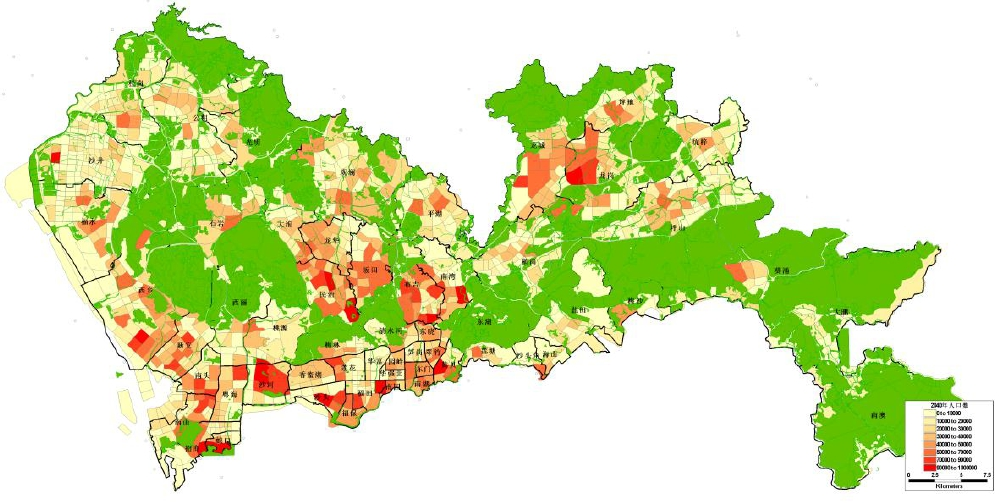
\includegraphics[width=\textwidth]{chp04_远期交通小区人口数.jpg}
  \caption{远期交通小区人口数\label{fig:chp04_远期交通小区人口数} }
\end{figure}

\subsection{对外交通量更新}
\subsubsection{口岸客运量}
2018 年,深港跨界客流平均每日约 67.6 万人次。自 2015 年 4 月起,深圳停
止签发居民“一签多行”签证而改为签发“一周一行”签证, 2018 日均总量比
2014 年的 63.3 万仅增长约 1.7\%。

\begin{figure}[!ht]
  \centering
  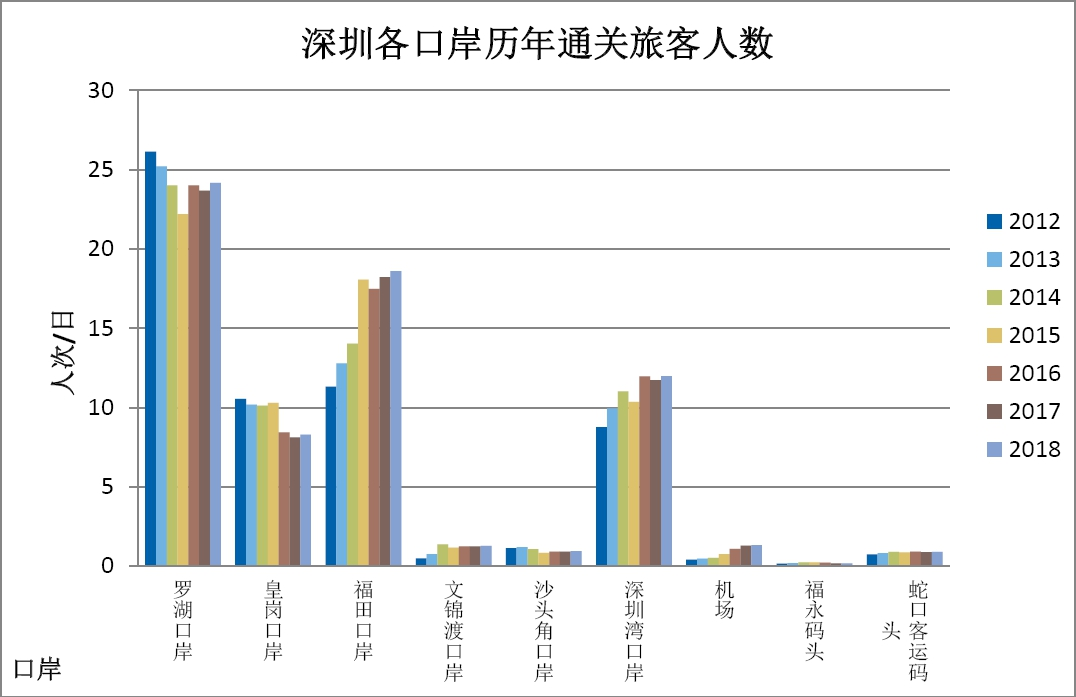
\includegraphics[width=\textwidth]{chp04_深港跨界日均通关旅客人次.jpg}
  \caption{深港跨界日均通关旅客人次 \protect\footnotemark\label{fig:chp04_深港跨界日均通关旅客人次}}
\end{figure}
\footnotetext{{2016 年数据来源于深圳边防检查总站提供 10 月的一周数据及 10 月 15 日--11 月 15日一月总的数据, 2015 年来源香港北来南往报告, 2014 年及以前来源 2014 深港莞惠跨界交通调查。}}

%\addtocounter{footnote}{-1}
\subsubsection{铁路客运量}
2017 年深圳市铁路发送量达到 7042 万人次/年,日均 19.3 万,比上年增长
6.4\%。按一般日统计,深圳市日均铁路发送量约 19.3 万人次,双向运输量约 38.6万人次。\clearpage

\begin{figure}[!ht]
  \centering
  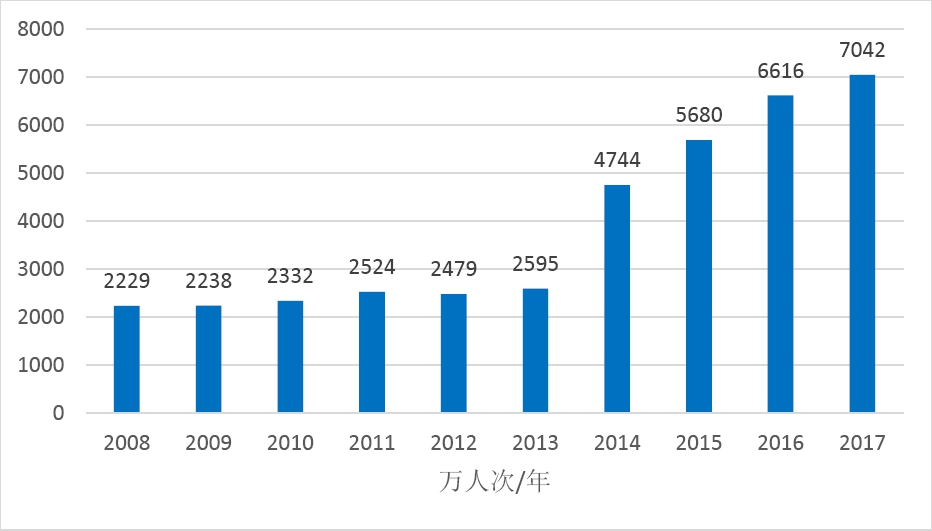
\includegraphics[width=0.9\textwidth]{chp04_历年深圳市铁路发送量统计情况图.jpg}
  \caption{历年深圳市铁路发送量统计情况图 \protect\footnotemark} \label{fig:chp04_历年深圳市铁路发送量统计情况图}
\end{figure}
\footnotetext{数据来源于深圳市统计年鉴}

深圳北站承担了铁路客运主体地位,客运量占比 58\%。福田站 15 年 12 月
30 日启用,客运量承担 7\%,客运量已在铁路站中排名第三。

\begin{table}[!ht]
\renewcommand{\arraystretch}{0.8} \centering
\caption[各铁路站历年发送量统计情况表]{各铁路站历年发送量统计情况表(万人次/年)\protect\footnotemark
\label{tbl:各铁路站历年发送量统计情况表}}
\begin{tabular} {|C{0.14\textwidth}|C{0.08\textwidth}|C{0.08\textwidth}|C{0.08\textwidth}|
C{0.08\textwidth}|C{0.08\textwidth}|C{0.08\textwidth}|C{0.09\textwidth}|}
  \hline
  \multicolumn{1}{|c|}{\bfseries 站名} & \multicolumn{1}{c|}{\bfseries 2011年} & 
  \multicolumn{1}{c|}{\bfseries 2012年} & \multicolumn{1}{c|}{\bfseries 2013年} & 
  \multicolumn{1}{c|}{\bfseries 2014年} & \multicolumn{1}{c|}{\bfseries 2015年} &
  \multicolumn{1}{c|}{\bfseries 2016年} & \multicolumn{1}{c|}{\bfseries 2017年} \\\hline

深圳北站 & 0 & 4.8 & 555 & 2093 & 3080 & 3610 & 4119 \\\hline
罗湖火车站 & 2144 & 1974 & 1991 & 1920 & 1727 & 1687 & 1758 \\\hline
福田站 & 0 & 0 & 0 & 0 & 0 & 113 & 482 \\\hline
光明站 & 0.3 & 25 & 28 & 37 & 56 & 72 & 87 \\\hline
坪山新站 & 0 & 0 & 0.3 & 34 & 52 & 70 & 103 \\\hline
深圳东站 & 0 & 3 & 201 & 261 & 292 & 340 & 328 \\\hline
深圳西站 & 340 & 306 & 244 & 258 & 216 & 150 & 100 \\\hline
\end{tabular}
\end{table}
\footnotetext{数据来源于铁路票务统计数据, 2017 年数据根据总量和 2018 年 5 月各站比例推算}

\subsubsection{航空客运量}
深圳机场 2017 年全年运送旅客达 4633 万人次,日均运送旅客量 12.7 万人,
比去年增长 6.4\%,客运量排名全国第五。

\begin{figure}[!ht]
  \centering
  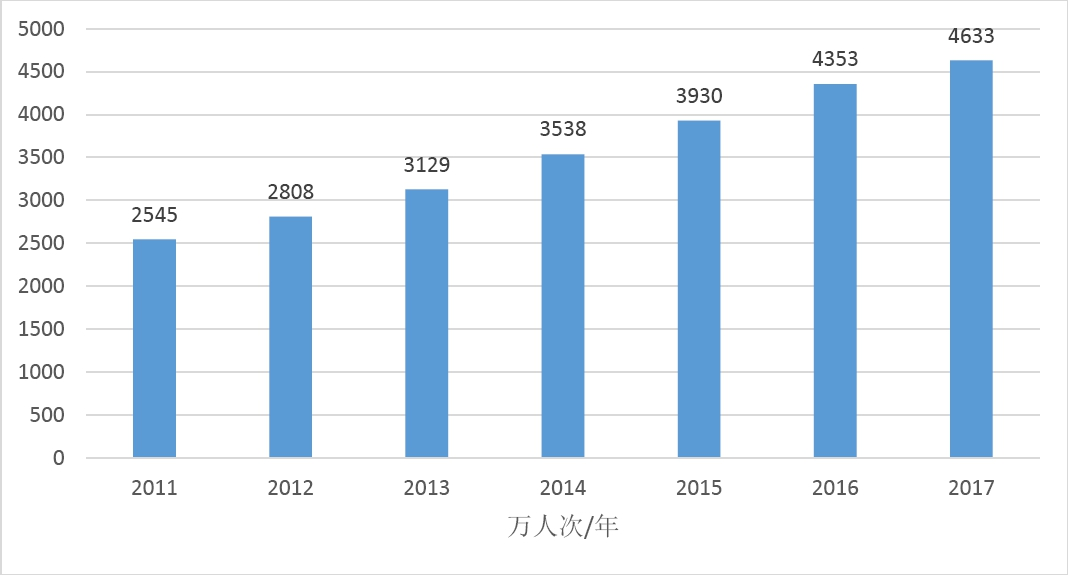
\includegraphics[width=0.9\textwidth]{chp04_历年机场旅客运输量.jpg}
  \caption{历年机场旅客运输量\label{fig:chp04_历年机场旅客运输量} }
\end{figure}

\subsubsection{长途客运站客运量}
根据深圳市统计公报, 2017 年全年公路运送旅客达 6001 万人次,比上年增
加 7.4\%,公路客运量有所回升。 2017 年公路日均发送 16.4 万人,双向运输量约
32.8 万, 2015 年公路运输日均运输量达到最高峰,为 18.0 万人次/日。

\begin{figure}[!ht]
  \centering
  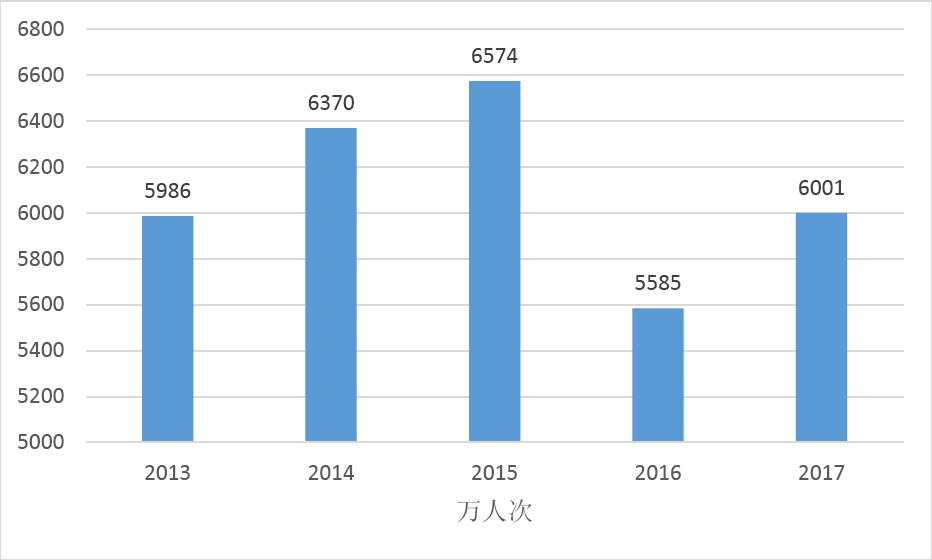
\includegraphics[width=0.9\textwidth]{chp04_历年公路运输量图.jpg}
  \caption{历年公路运输量图\label{fig:chp04_历年公路运输量图} }
\end{figure}

深圳长途汽车客运量中罗湖客运站占比最大,约 31\%,其余均小于 10\%。
原特区外较多街道级别的客运站客运量比例不足 1\%。

\subsubsection{对外主要道路客运量}
深莞惠边界道路客流量呈平稳增长趋势,客流总量为 184.3 万人次/日。其中,
深莞边界全天双向客流总量为 138 万人次/日,相比 2016 年的 130.2 万人次/日,
增长 6.0\%;深惠边界全天双向客流总量为 46.3 万人次/日,相比 2016 年的 38.0
万人次/日,增长 21.8\%, 增幅较大。

\begin{figure}[!ht]
  \centering
  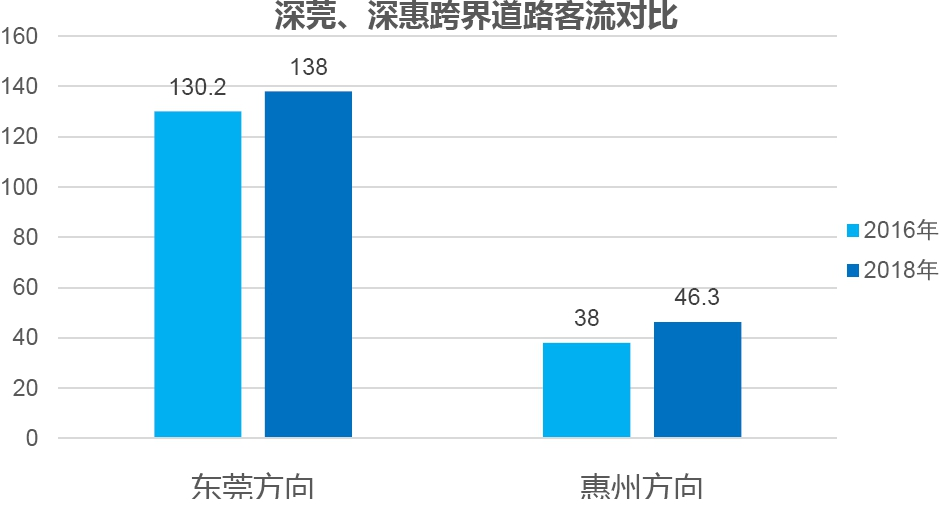
\includegraphics[width=0.9\textwidth]{chp04_深莞惠边界客流总量图.jpg}
  \caption{深莞惠边界客流总量图\label{fig:chp04_深莞惠边界客流总量图} }
\end{figure}

\renewcommand{\arraystretch}{0.8}
\begin{longtable}[c] {|C{0.1\textwidth}|C{0.15\textwidth}|C{0.15\textwidth}|C{0.15\textwidth}|}
  \caption[现状及规划年主要对外通道客流量]{现状及规划年主要对外通道客流量(单位:万人次/日)
\label{tbl:现状及规划年主要对外通道客流量}}
  \hline
  \multicolumn{1}{|c|}{\bfseries 方向} & \multicolumn{1}{c|}{\bfseries 道路名称} & 
  \multicolumn{1}{c|}{\bfseries 2018 年} & \multicolumn{1}{c|}{\bfseries 2040 年}\\\hline

西 & 江湾大道 & 0.0 & 20.7\\\hline
西 & 沿江高速 & 13.4 & 20.\\\hline
西 & 广深高速 & 27.0 & 20.\\\hline
西 & 广深公路 & 13.8 & 12.\\\hline
西 & 根玉路 & 0.0 & 15.5  \\\hline
西 & 龙大高速 & 14.8 & 15.\\\hline
西 & 公常公路 & 4.5 & 9.5 \\\hline
中 & 深华快速 & 0.0 & 13.8\\\hline
中 & 梅观高速 & 19.6 & 13.\\\hline
中 & 沙湖大道 & 1.9 & 1.9 \\\hline
中 & 四联路 & 1.5 & 1.5   \\\hline
中 & 泗黎路 & 3.5 & 9.5   \\\hline
中 & 清平快速 & 0.0 & 13.8\\\hline
中 & 高尔夫大道 & 6.4 & 9.\\\hline
中 & 平龙西路 & 9.6 & 4.3 \\\hline
中 & 东深公路 & 5.4 & 9.5 \\\hline
中 & 龙平西路 & 8.3 & 4.3 \\\hline
中 & 博深高速 & 7.4 & 15.5\\\hline
中 & 如意路 & 3.4 & 1.7   \\\hline
中 & 祥新西路 & 2.1 & 1.7 \\\hline
东 & 坪西快速 & 0.0 & 13.8\\\hline
东 & 深惠高速 & 5.9 & 15.5\\\hline
东 & 深惠公路 & 4.0 & 9.5 \\\hline
东 & 锦绣东路 & 2.4 & 3.0 \\\hline
东 & 乌石路 & 4.2 & 4.6   \\\hline
东 & 深汕高速 & 9.4 & 15.5\\\hline
东 & 深汕公路 & 4.9 & 9.5 \\\hline
东 & 丹梓路 & 2.9 & 6.3   \\\hline
东 & 兰竹路 & 3.7 & 4.6   \\\hline
东 & 盐坝高速 & 4.4 & 10.3\\\hline
\multicolumn{2}{|c|}{合计} & 184.3 & 308.4 \\\hline
\end{longtable}

\subsection{输入数据更新流程}
基础输入数据,在检查自定义属性已经建好后,可以直接在小区列表中更新,
更多的是在 Excel 表格中对于数据进行编辑和更新。

对于常用的人口、用地和特殊吸引点流量数据,通过 Updating Planning
Data.vbs 页面的数据。

\begin{nbeae}
\item 更新“PlanningData”页面的数据并保存,数据包括家庭户人、集体户
人口、一类住宅、二类及以下住宅、行政办公、教育科研、中小学、其他公共用
地、商业用地、工业用地、仓储用地、其他用地、交通用地、岗位数、入境小汽
车(车)、离境小汽车(车)、入境货车(车)、离境货车(车)、入境公交(人)、
离境公交(人)这 20 项内容。其中后面六个属性只针对特殊吸引点小区,即小区编号大于 
9000 的小区(见图\ref{fig:chp04_更新PlanningData页面数据});

\begin{figure}[!ht]
  \centering
  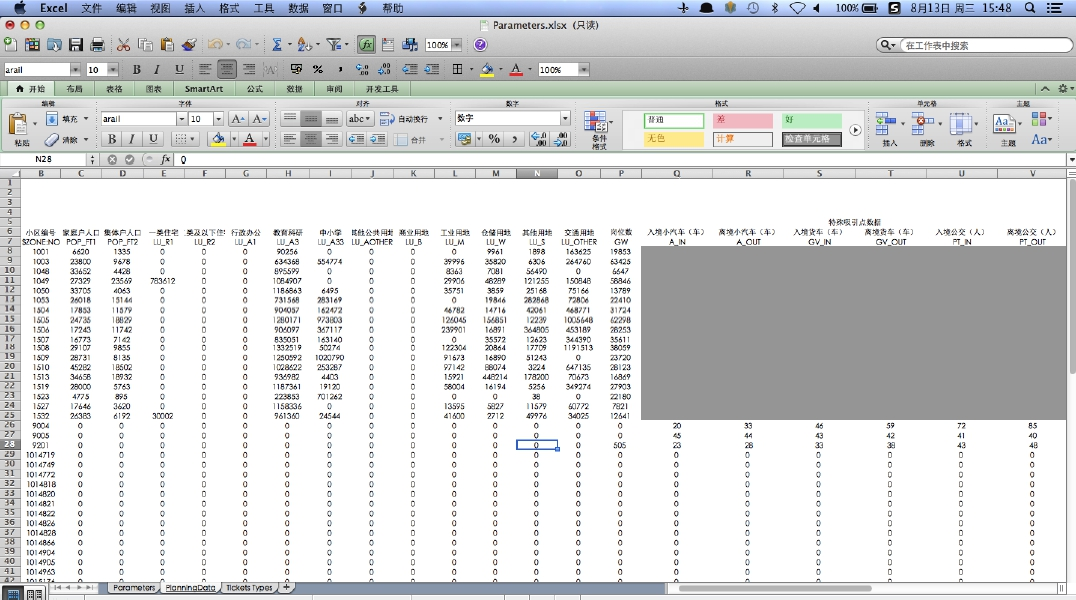
\includegraphics[width=\textwidth]{chp04_输入数据更新1.jpg}
  \caption{更新PlanningData页面数据\label{fig:chp04_更新PlanningData页面数据} }
\end{figure}

\item 第二步,保持 Parameters.xlsx 运行 Updating Planning Data.vbs,
由程序自动读取 Excel 中数据,更新小区输入数据(见图\ref{fig:chp04_更新小区输入数据})。

\begin{figure}[!ht]
  \centering
  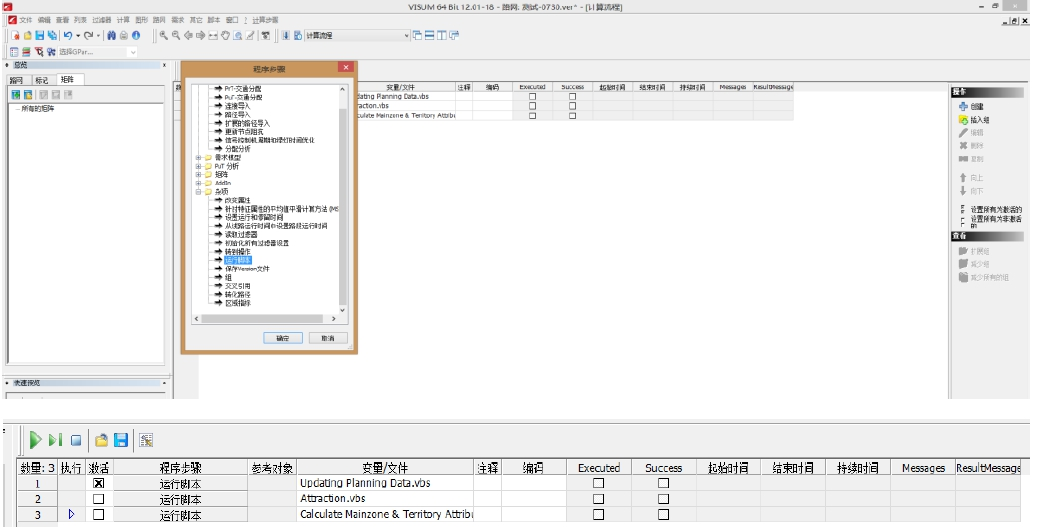
\includegraphics[width=\textwidth]{chp04_更新小区输入数据.jpg}
  \caption{更新小区输入数据\label{fig:chp04_更新小区输入数据} }
\end{figure}
\end{nbeae}

除了预设的常用人口和用地数据更新,其他数据也可以通过复制到 Excel
批量修改后粘贴回去进行较便捷的更新操作:
\begin{nbeae}
\item 选择列表属性,并拷列表进入 Excel 做为数据输入模板;
\item 在 Excel 中更新数据。 打开 Excel 表格,选取 A1 单元格,右键粘贴;
选择需要修改的属性进行更新,注意属性名称行上面的行为 visum 识别的标头不能改动。更新完毕后,选择整个工作表进行复制;
\item 在 VISUM 小区列表中黏贴 Excel 的数据,见图\ref{fig:chp04_更新VISUM中的输入数据}。
\end{nbeae}

\begin{figure}[!ht]
  \centering
  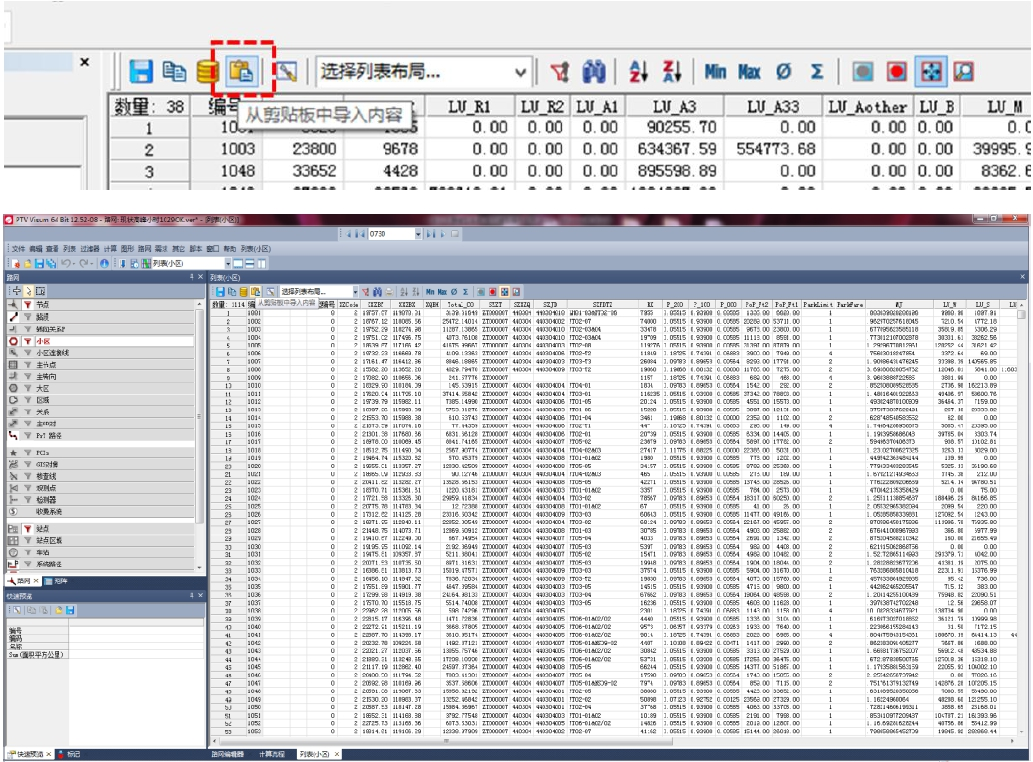
\includegraphics[width=\textwidth]{chp04_更新VISUM中的输入数据.jpg}
  \caption{更新VISUM中的输入数据\label{fig:chp04_更新VISUM中的输入数据} }
\end{figure}

\section{模型优化及矩阵更新}
\subsection{模型优化思路}
传统模型参数的优化及校核主要依赖于居民出行调查,一般五年更新一次。
本次模型更新基于 2016 年居民出行调查数据,结合模型应用需求,对收入及拥
车模型、发生吸引模型架构进行优化,对参数进行重新校核。此外根据公交、轨
道刷卡数据、 GPS 数据等动态多源大数据更新现状矩阵。

\subsection{收入模型更新}
既有收入模型分两步,第一步预测各区平均收入,第二步预测小区平均收入。
考虑收入模型主要用来预测拥车,而单一的平均收入水平指标不能完全反映小区的拥车水平。

不同收入水平与其拥车数量存在较高的相关性,如年收入 30 万以上的家庭
80\%为有车户,因此预测小区收入分布比小区平均收入更能反映拥车的真实情况,
香港的模型也采用预测小区收入分布的方式。

既有模型中小区平均收入影响因素为集体户比例及人均住房面积。根据
2016 年居民出行调查结果显示,集体户比例已由 30\%下降至 20\%。中心区及二
圈层片区集体户比例已接近,对收入差距的反映不明显。 基于建筑物普查的人均
住房面积,在小区层面数据看离散度高,差异较大,与收入拟合度差。

考虑到工业比例较高的片区,收入相对较低;距离中心区越近,收入相对越
高;另外也研究了各类型用地、不同容积率等等因素与平均收入的关系,拟合度
均比较差,因此通过现状土地利用及区位来拟合平均收入,基本不可行。图\ref{fig:chp04_交通小区平均收入分布图}
是经过调整后的交通小区平均收入分布图。

\begin{figure}[!ht]
  \centering
  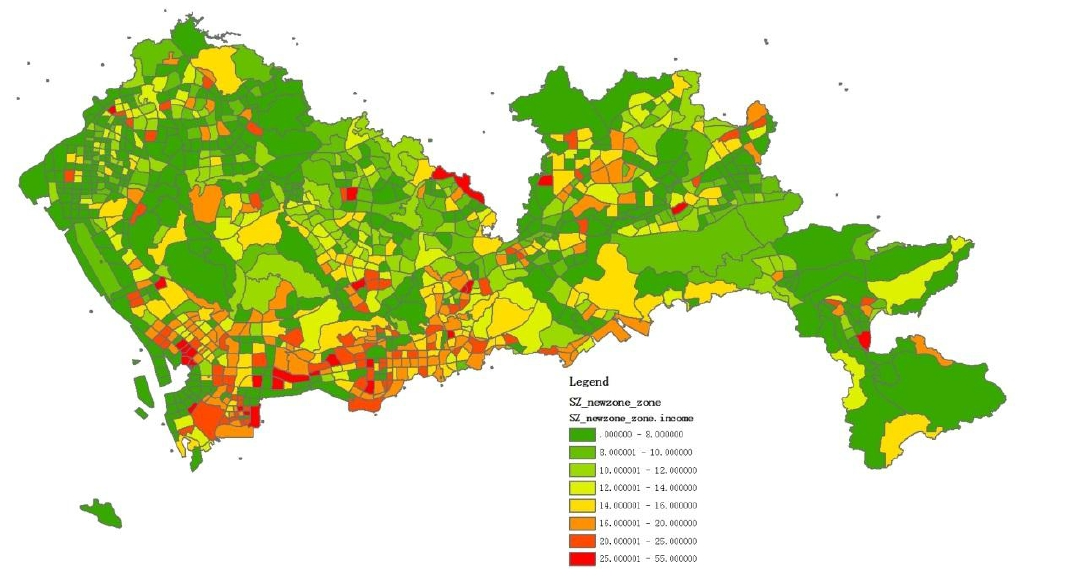
\includegraphics[width=\textwidth]{chp04_交通小区平均收入分布图.jpg}
  \caption{交通小区平均收入分布图\label{fig:chp04_交通小区平均收入分布图} }
\end{figure}


考虑到规划模型需要一定的定性判断和假设,例如大空港片区,可能发展为
未来新的全市性就业中心,但并未有与之定位相对应的详细规划。因此,考虑借
用发生吸引强度系数,综合表达每个交通小区的定位。全市发生、吸引强度系数
分为 1-8 个等级,参考既有调查得到的发生吸引强度,并综合考虑区位、地铁等
因素。1 类表示全市性的就业中心或高密度成熟居住区域,2 基本为片区级中心,
3 为轨道站点区域,以此类推, 8 为公园绿地等人口岗位密度最低的片区。图\ref{fig:chp04_机动化出行发生强度分布图}
和图\ref{fig:chp04_机动化出行吸引强度分布图}分别是调整后的机动化出行发生强度和吸引强度分布图。

\begin{figure}[!ht]
  \centering
  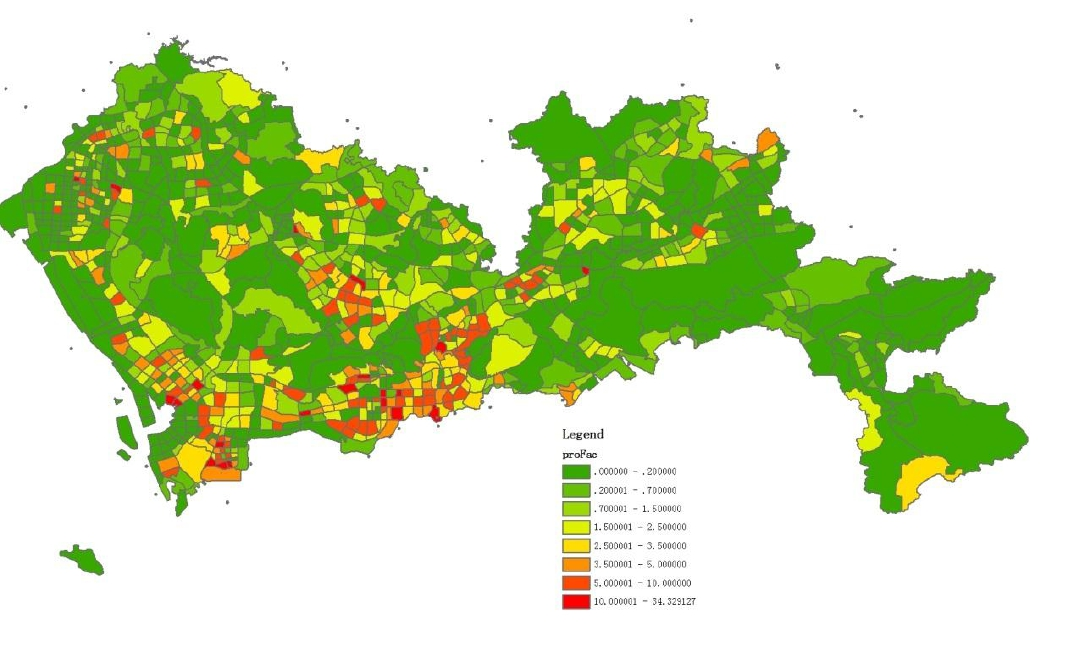
\includegraphics[width=\textwidth]{chp04_机动化出行发生强度分布图.jpg}
  \caption{机动化出行发生强度分布图\label{fig:chp04_机动化出行发生强度分布图} }
\end{figure}

\begin{figure}[!ht]
  \centering
  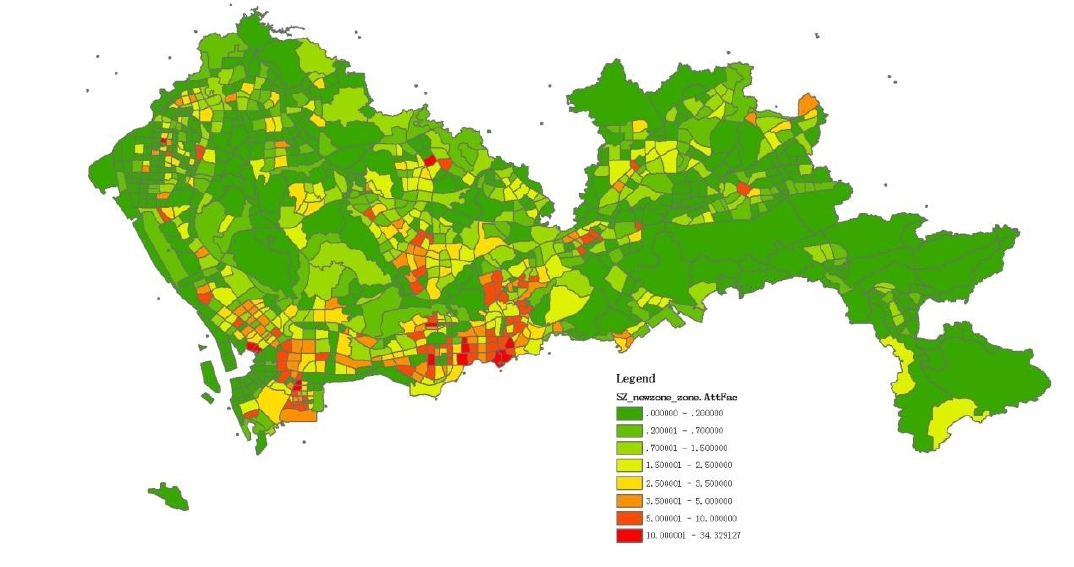
\includegraphics[width=\textwidth]{chp04_机动化出行吸引强度分布图.jpg}
  \caption{机动化出行吸引强度分布图\label{fig:chp04_机动化出行吸引强度分布图} }
\end{figure}

既有调查小区总共包含 701 个小区的家庭收入信息,筛除样本数小于 30 的
小区,共 448 个有效小区数据。按照调查,收入分为 5 类: <10 万、 10-20 万、
20-30 万、 30-50 万、 >50 万。考虑到 30 万以上比例较低,因此将 30-50 万和>50
万进行合并,分为四个收入等级。

\begin{equation}
每个小区各类收入的比Inci=发生系数\times a_i+吸引系数\times b_i + c_i
\end{equation}

根据既有调查数据,得到不同发生吸引强度下各类收入比例,参数值如表\ref{tbl:收入模型参数值}所示:

\renewcommand{\arraystretch}{0.8}
\begin{longtable}[c] {|C{0.15\textwidth}|C{0.15\textwidth}|C{0.15\textwidth}|}
  \caption{收入模型参数值\label{tbl:收入模型参数值}}
  \hline
  \multicolumn{1}{|c|}{\bfseries 收入等级} & \multicolumn{1}{c|}{\bfseries 参数} &
  \multicolumn{1}{c|}{\bfseries 参数值} \\\hline

  \multirow[c]{3}*{<10万} & $a_1$ & -0.0528 \\\cline{2-3}
  & $b_1$ & 0.0741 \\\cline{2-3}
  & $c_1$ & 0.0472 \\\hline
  \multirow[c]{3}*{10--20 万} & $a_2$ & -0.0528 \\\cline{2-3}
  & $b_2$ & 0.0741 \\\cline{2-3}
  & $c_2$ & 0.0472 \\\hline 
  \multirow[c]{3}*{20--30 万} & $a_3$ & -0.0121 \\\cline{2-3}
  & $b_3$ & -0.0060 \\\cline{2-3}
  & $c_3$ & 0.3220 \\\hline
  \multirow[c]{3}*{>30 万} & $a_4$ & -0.0009 \\\cline{2-3}
  & $b_4$ & -0.0076 \\\cline{2-3}
  & $c_4$ & 0.0917 \\\hline 
\end{longtable}

\subsection{收入及拥车模型更新}
收入模型用以计算小区中 NCO(不拥车家庭)比例, CO1(拥有一辆车家
庭)比例,和 CO2(拥有两辆及以上车家庭)比例;并且根据小区总家庭数可
以计算小区 NCO 家庭数、 CO1 家庭数、 CO2 家庭数,以及小区车辆拥有数。

既有的交通模型为双层 Logit 模型。 其公式如下:

\begin{flalign}
&P(1+)_i = 1/(1 + exp(a + b\times I_i + c\times log(I_i) + f(park))) \\
&P(2+)_i = 1/(1 + exp(a + b\times I_i + c\times log(I_i)))
\end{flalign}


\noindent{其中:}
\begin{para}
\item[$P(1+)_i$]:第$i$小区拥有一辆及以上车的家庭比率
\item[$P(2+)_i$]:第$i$小区拥有两辆及以上车的家庭比率
\item[$I_i$]:第$i$小区的家庭平均收入
\item[$f(park)$]:停车惩罚量
\end{para}

既有模型构建网络中仅有 22 公里轨道网络,轨道可达性对拥车影响不大。
但 2016 年 11 月开展居民出行调查时,全市已开通 268 公里轨道网络, 覆盖了
中心城区及二圈层片区, 轨道网络可达性大大提高,对拥车产生一定影响。

本次拥车模型采用分类方法,综合考虑收入、轨道、拥车三个因素,得出各
类型拥车比例如表\ref{tbl:拥车模型分类值}所示。

\begingroup
\zihao{5}
\renewcommand{\arraystretch}{0.8}
\begin{longtable}[c] {|C{0.08\textwidth}|C{0.07\textwidth}|B{0.12\textwidth}|B{0.12\textwidth}|C{0.06\textwidth}|
B{0.12\textwidth}|B{0.12\textwidth}|C{0.06\textwidth}|}
  \caption{拥车模型分类值\label{tbl:拥车模型分类值}}
  \hline
  \multirow[c]{3}{*}{\parbox{\linewidth}{\bfseries Income}} & \multirow[c]{3}{*}{\parbox{\linewidth}{\bfseries Car Owner}} &
  \multicolumn{3}{c|}{\bfseries 无轨道} & \multicolumn{3}{c|}{\bfseries 有轨道} \\ \cline{3-8}

  & & {\bfseries 原特区外/ 停车无限制} & {\bfseries 原特区内/ 停车限制} & {\bfseries 总体} & 
{\bfseries 原特区外/ 停车无限制} & {\bfseries 原特区内/ 停车限制} & {\bfseries 总体} \\\hline
\multirow{3}*{<10 万} & NCO & 90\% & 71\% & 89\% & 81\% & 77\% & 79\% \\\cline{2-8}
& CO1 & 10\% & 28\% & 10\% & 19\% & 22\% & 20\% \\\cline{2-8}
& CO2 & 0\% & 0\% & 0\% & 0\% & 1\% & 1\% \\\hline
\multirow{3}*{10--20万} & NCO & 69\% & 49\% & 68\% & 59\% & 52\% & 55\% \\\cline{2-8}
& CO1 & 30\% & 50\% & 31\% & 39\% & 46\% & 43\% \\\cline{2-8}
& CO2 & 1\% & 2\% & 1\% & 2\% & 2\% & 2\% \\\hline
\multirow{3}*{20--30万} & NCO & 30\% & 14\% & 29\% & 27\% & 21\% & 23\% \\\cline{2-8}
& CO1 & 65\% & 78\% & 67\% & 67\% & 73\% & 71\% \\\cline{2-8}
& CO2 & 4\% & 8\% & 5\% & 6\% & 5\% & 6\% \\\hline
\multirow{3}*{>30 万} & NCO & 18\% & 14\% & 18\% & 16\% & 5\% & 10\% \\\cline{2-8}
& CO1 & 73\% & 78\% & 73\% & 72\% & 80\% & 77\% \\\cline{2-8}
& CO2 & 9\% & 8\% & 9\% & 12\% & 15\% & 14\% \\\hline
\end{longtable}
\endgroup

\subsection{发生吸引模型更新}
发生吸引模型是四阶段模型的第一步,即计算交通小区的发生量及吸引量。
发生模型一般采用交叉分类法,吸引模型采用回归分析法。发生吸引模型一般根
据户特征、人特征以及出行目的,分为多类。本次更新在人群分类、出行目的分
类、区域分类方面均做了更新。

\begin{nbeae}
\item 增加机动化出行发生及吸引量计算。考虑到宏观模型应用主要面向道
路及公共交通评估,即机动化出行需求,因此本次发生吸引模型在发生吸引阶段,
在以往全方式出行量基础上,补充机动化出行量;
\item 关于人群分类, 结合收入和拥车,将家庭户分为高、中高、 中低、低收入四类;
\item 出行目的合并为 6 大类。由于原先出行目的分类中基于家的购物娱乐
出行及基于家的私人出行比例较小,因此对这两类目的进行合并。出行目的分为
基于家的工作出行( HBW)、基于家的上学出行( HBE)、基于家的购物娱乐出
行( HBS)、基于家的其他出行( HBO)、商务出行( EB)、非基于家的工作出行
( NHW)共六类;
\item 分区域拟合发生吸引模型参数。由于全市产业结构及人口结构差异较
大,不同片区人口出行率及用地吸引率差别较大,因此将全市分为多个区域分别
拟合模型参数,以提高模型预测精度。结合产业结构分布、人均出行率等指标,
发现空间呈现较为明显的三圈层结构,即罗湖-福田-南山中心城区,盐田以及原
原特区外至机荷高速的二圈层片区,以及更远的三圈层片区。发生吸引模型均按
照三个圈层进行参数校核,表\ref{tbl:chp04_出行发生模型参数}和表
\ref{tbl:chp04_出行吸引模型参数}是参数拟合结果;
\item 引入发生吸引强度系数。 一方面,核心就业片区发生吸引强大明显高
于其他片区,另一方面详细规划土地利用往往滞后于宏观规划。为能更好评估重
点片区交通需求,引入发生吸引强度系数,为规划多方案测试提供支撑。
\end{nbeae}

\begin{table}[!ht]\centering
\caption{出行发生模型参数\label{tbl:chp04_出行发生模型参数}}
\begin{tabularx}{\textwidth}{@{\extracolsep{\fill}}*{1}{c}@{}}
  \centering{
  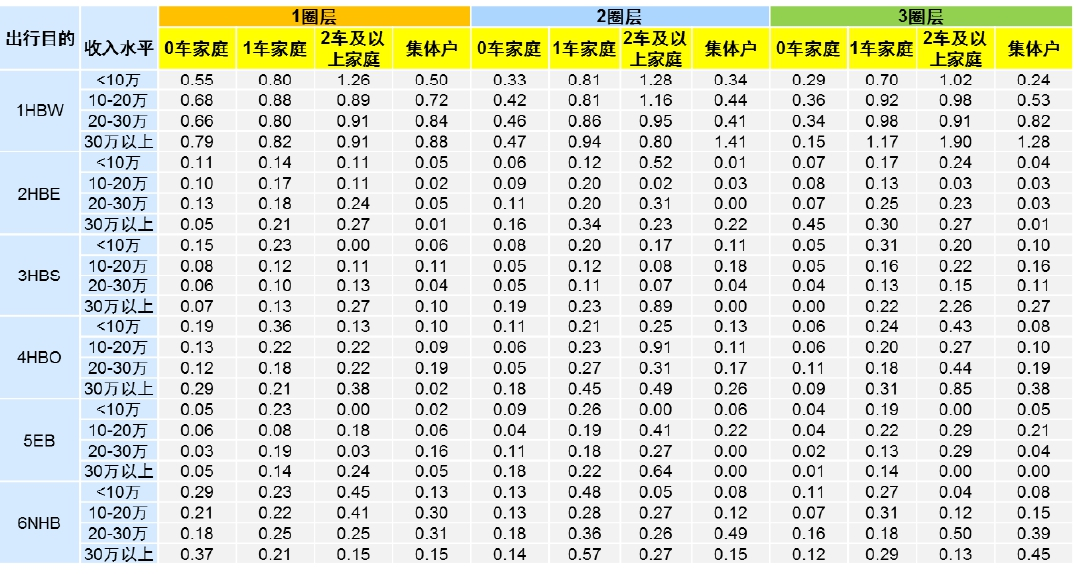
\includegraphics[width=\textwidth]{chp04_出行发生模型参数.jpg}}
\end{tabularx}
\end{table}

\begin{table}[!ht]\centering
\caption{出行吸引模型参数\label{tbl:chp04_出行吸引模型参数}}
\begin{tabularx}{0.75\textwidth}{@{\extracolsep{\fill}}*{1}{c}@{}}
  \centering{
  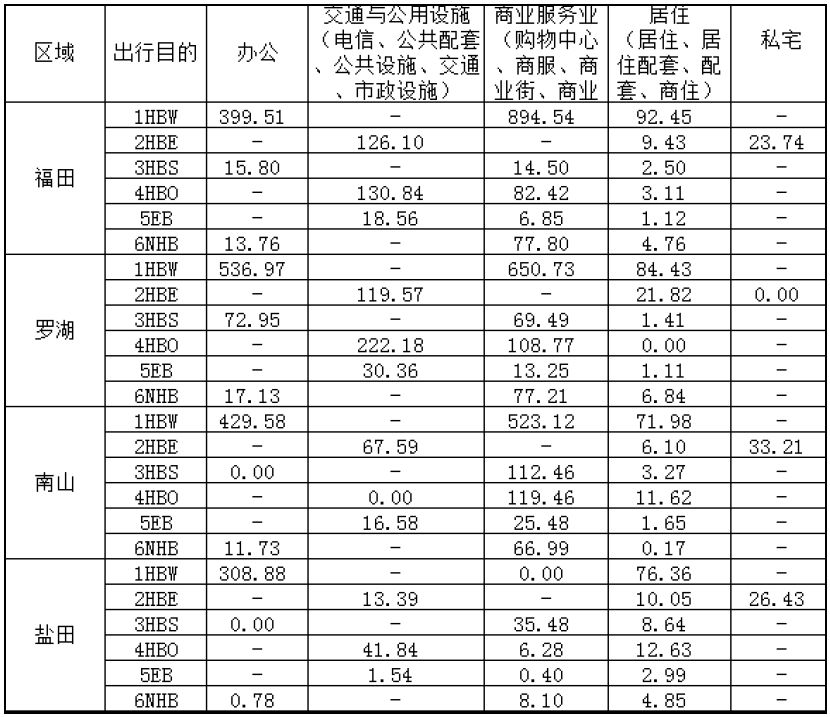
\includegraphics[width=0.75\textwidth]{chp04_出行吸引模型参数.jpg}}
\end{tabularx}
\end{table}

\subsection{矩阵更新}
\subsubsection{客运量变化}
2016 年,公共交通日均客运量为 966 万人次,其中,轨道交通客运总量为
354 万人次,常规公交为 510 万人次,出租车客运量为 102 万人次。2012 年以来,
公共交通客运量基本维持在 1000 万人次/日上下, 2014 年达到了历年高点,为
1023 万人次/日。从出行结构看,随着轨道交通线网的完善,轨道交通客运量逐
年攀升,相应的常规公交、出租车的出行比例均在下降, 2016 年轨道交通、常
规公交、出租车在公共交通中的比重分别为 36.6\%、 52.8\%、 10.6\%。

\begin{figure}[!ht]
  \centering
  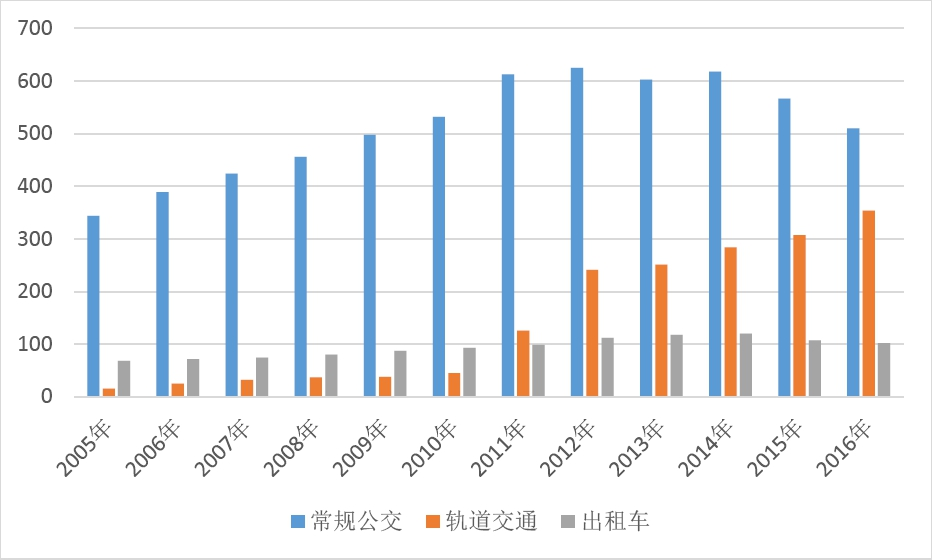
\includegraphics[width=0.8\textwidth]{chp04_历年公交方式客流量.jpg}
  \caption{历年公交方式客流量\label{fig:chp04_历年公交方式客流量} }
\end{figure}

\subsubsection{轨道大区分布及变化}
特区内行政区对周边的特区外行政区有较强的辐射力, 东中西轴向通道的客
流量持续增强,宝安区与南山区、 龙华与福田、龙岗与罗湖的联系较为紧密。

\begin{figure}[!ht]
  \centering
  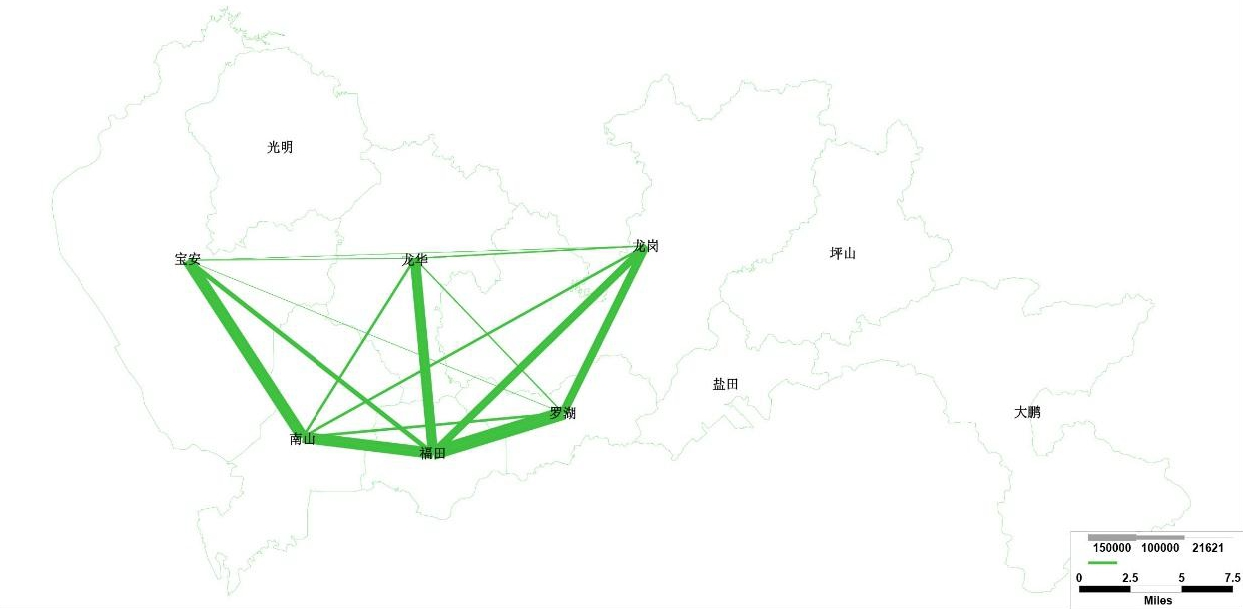
\includegraphics[width=\textwidth]{chp04_全市行政区轨道出行OD分布.jpg}
  \caption{全市行政区轨道出行OD分布\label{fig:chp04_全市行政区轨道出行OD分布} }
\end{figure}

\subsubsection{常规公交大区分布及变化}
常规公交大区 OD 联系的紧密程度与轨道大区 OD 有相似之处, 但是中龙华-
龙岗之间的常规公交联系明显强于其轨道联系,原因是目前龙华与龙岗之间没有
直达的轨道, 使用轨道的效率较低,随着轨网的进一步建设客流可能发生转移。

\begin{figure}[!ht]
  \centering
  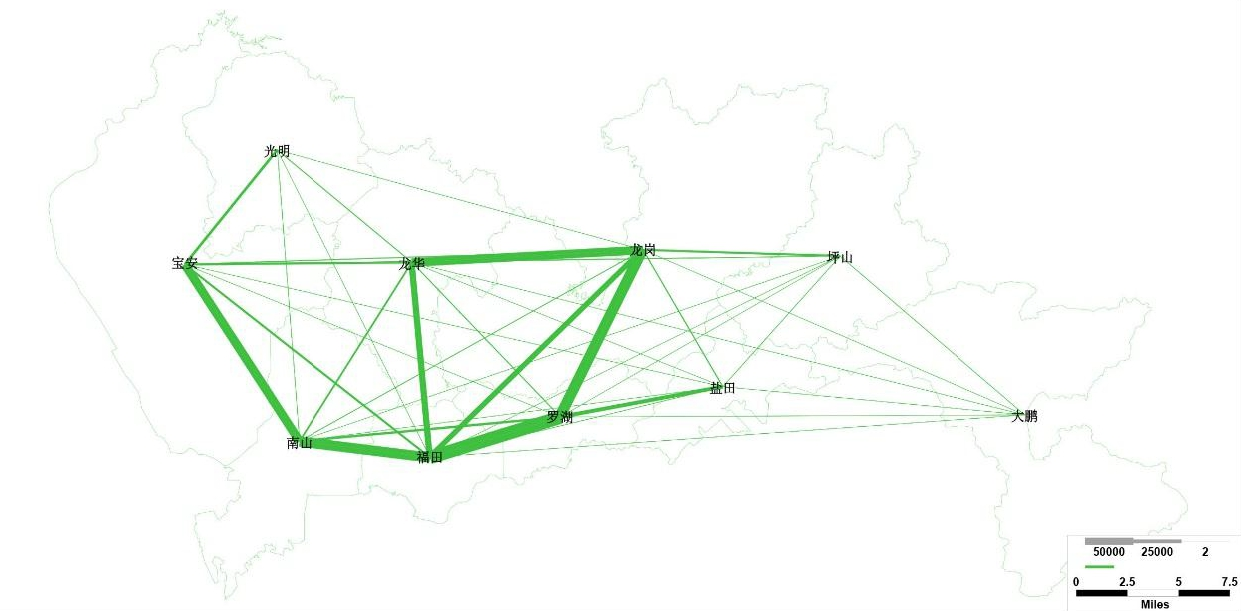
\includegraphics[width=\textwidth]{chp04_全市行政区常规公交出行OD分布.jpg}
  \caption{全市行政区常规公交出行OD分布\label{fig:chp04_全市行政区常规公交出行OD分布} }
\end{figure}

\subsubsection{出租车大区分布及变化}
出租车的出行量相对较少,而且跨区联系中以罗湖-福田的联系为主, 其他
联系相对较弱。

\begin{figure}[!ht]
  \centering
  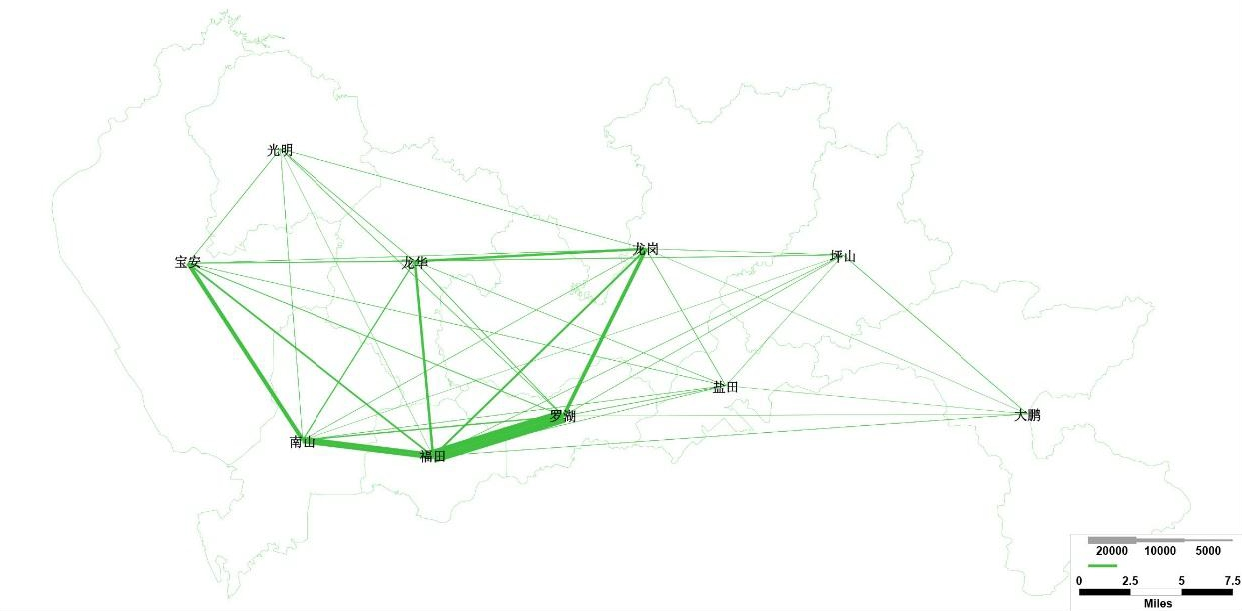
\includegraphics[width=\textwidth]{chp04_全市行政区出租车出行OD分布.jpg}
  \caption{全市行政区出租车出行OD分布\label{fig:chp04_全市行政区出租车出行OD分布} }
\end{figure}

\section{模型更新主要成果}
\subsection{人口及岗位分布}
\smalltitle{现状人口岗位分布}










